\begin{savequote}[45mm]
Gauge symmetry principles are regularly invoked in the context of justification, as deep physical principles, fundamental starting points in thinking about why physical theories are the way they are, so to speak.  
\qauthor{Christopher A. Martin}
\end{savequote}
\chapter{Gauge Theories}
\section{Global Gauge Invariance}

 \begin{figure}[h!]
    \centering
    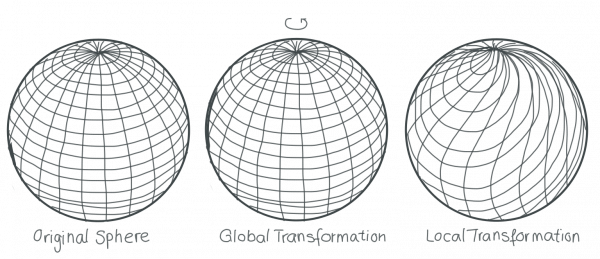
\includegraphics{Figures/localtransformations.png}
    \caption{Gauge Transformations represented pictorially}
    \label{fig:my_label}
\end{figure}

\section{Local Gauge Invariance}

 \begin{figure}
    \centering
    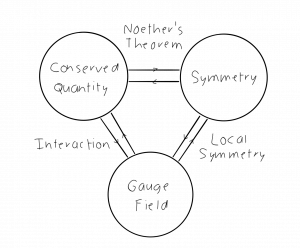
\includegraphics{Figures/gaugetheornoether.png}
    \caption{Noether's Theorem and Gauge Fields}
    \label{fig:my_label}
\end{figure}

\subsection{Summary}
The Gauge transformation only alters the phase of the field globally
Since the generator of time translations the invariance of the functional implies the invariance of the Lagrangian to the first order in $\epsilon$
\begin{equation}
    \mathcal{L} = \mathcal{L}^{'}
\end{equation}
This gives us the conservation law
\begin{equation}
 \partial_{\mu} j^{\mu} = 0
\end{equation}
where $j^{\mu}$ is defined as
\begin{equation}
    j^{}
\end{equation}
\section{Electrodynamics as a Gauge Theory}

\section{Pure Electrodynamics, Spacetime Invariances and Conservation Laws}
Using the Lagrangian equation for electromagnetic fields, we build the electromagnetic canonical momentum tensor $P_{\rho \sigma}$ of the form, 
\begin{equation}
    P_{\rho \sigma } \equiv \frac {\delta \mathcal{L}}{\delta A^{\rho,\sigma}}
\end{equation}
\begin{equation}
    \frac{\delta (\delta ^{\rho} A^{\sigma})}{\delta (\delta ^{\mu} A^{\nu})} = \delta ^{\rho} _{\mu} \delta^{\sigma}_{\nu}
\end{equation}
Hence we can see that, 
\begin{equation}
    P_{\rho \sigma} = F_{\rho \sigma}
\end{equation}
We can define the Hamiltonian tensor for Pure electromagnetism as, 
\begin{gather}
   \mathcal{H}^{(A) \: \nu}_{\mu} = A^{\rho}_{\mu} P^{\nu}_{\rho}- \delta_{\mu}^{\nu} \mathcal{L}^{(A)} \\
 = (\delta_{\mu} A^{\rho} ) F_{\rho} ^{\nu} - \delta _{\mu}^{\nu} \mathcal{L}^{(A)}
\end{gather}
Now lets look at what happens when an infinitissimal change of $\epsilon$ is made on the spacetime coordinates, 
\begin{gather}
    x^{' \mu} = x^{\mu} + \epsilon  \tau^{\mu} \\
     A ^{' \mu} = A^{\mu} + \epsilon  \tau^{\mu}
\end{gather}
The condition for invariance is , 
\begin{equation}
    \mathcal{L}^{'} G = \mathcal{L} \approx \epsilon^{s}
\end{equation}
When "S>1", it is called as the Jacobian transformation. When this is differentiated with respect to $\epsilon$, and when $\epsilon$ is set to 0, we get the vector field version of fundamental invariance identity of Rund and Trautman, 
\begin{equation}
    -(\frac{\delta \mathcal{L}^{A}}{\delta A^{\mu}} - \delta_{\nu} P_{\mu}^{\nu}) (\mathcal{T}^{\mu} - A^{\mu}_{\sigma} \tau^{\sigma}) = \delta_{\nu}[P_{\rho}^{\nu} \mathcal{T}^{\rho} - \mathcal{H}^{A \: \: \nu}_{\rho} \tau^{\rho} ]
\end{equation}
The LHS becomes zero when it satisfies Euler-Lagrange equation. So if 'j' is invariant under the tranformation shown above, and if 'j' is necessarily an extremal, then equation (7.9) gives the Noether's theorem in the form of the continuity equation, 
\begin{equation}
    S^{\nu} \equiv P_{\rho} ^{\nu} \tau ^{\rho} - \mathcal{H}^{(A)\: \: \nu}_{\rho} \tau ^{\rho}
\end{equation}





\section{Internal Degrees of Freedom}
Internal degrees of freedom are the transformations that we can make between the fields themselves in the Lagrangian. For instance

\section{Non-Abelian Gauge Transformations}
Non-Abelian gauge transformations are simply those which form a non-abelian i.e. non-commutative group.

\subsection{The Kaon Toy Model}

